\section{Sheaf Cobordism on Inter-generator Regions}
Suppose we have a punctured Riemann sphere $M$ and $\Lambda_0^0$, $\Lambda_0^\infty$, $\Lambda_0^{squig}$, a nested regions $U\subset U' \subset M$, and a chart $f : U \rightarrow \R^2$ such that $U'$ maps to $R:=(-1,1)_x \times (-n-1,n+1)_z$ under $f$
\begin{itemize}
\item $\Lambda_0^0$ gets mapped to $\overset{n}{\underset{k=1}{\cup}}\{(x,z)\in R \mid z=\Psi(-k,n-k+\frac{1}{2})(x)\}$, co-oriented upward.

\item $\Lambda_0^\infty$ gets mapped to $\overset{n}{\underset{k=1}{\cup}}\{(x,z)\in R \mid z=k\}$, co-oriented downward.

\item $\Lambda_0^{squig}$ gets mapped to $\{(x,z)\in R \mid x=0\}$, co-oriented toward the left.
\end{itemize}
and a sheaf defined by the following squiggly legible diagram. All the maps corresponding to blue strands are $\iota_1$ and the red strands $\iota_0$ otherwise stated. I have omitted these maps from the diagram.\\

\begin{figure}[H]
    \centering
    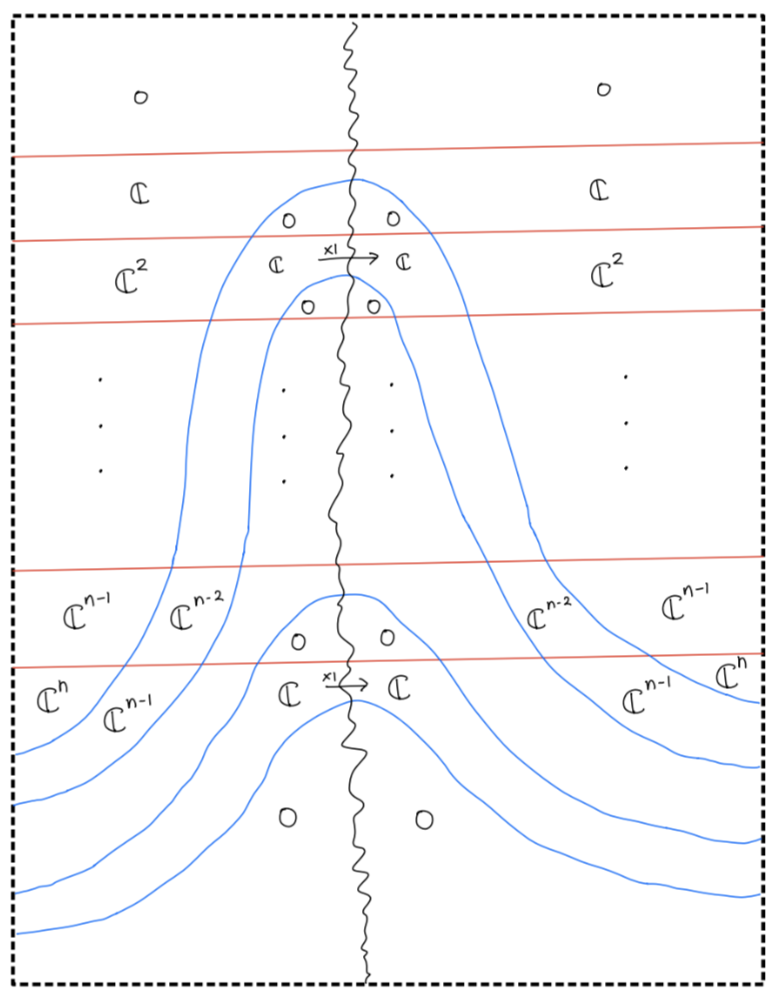
\includegraphics[scale = 0.95]{diagrams/cobord_inter/0.png}
    \caption{}
    \label{fig:your-label}
\end{figure}
\pagebreak
which is quasi-isomorphic to

\begin{figure}[H]
    \centering
    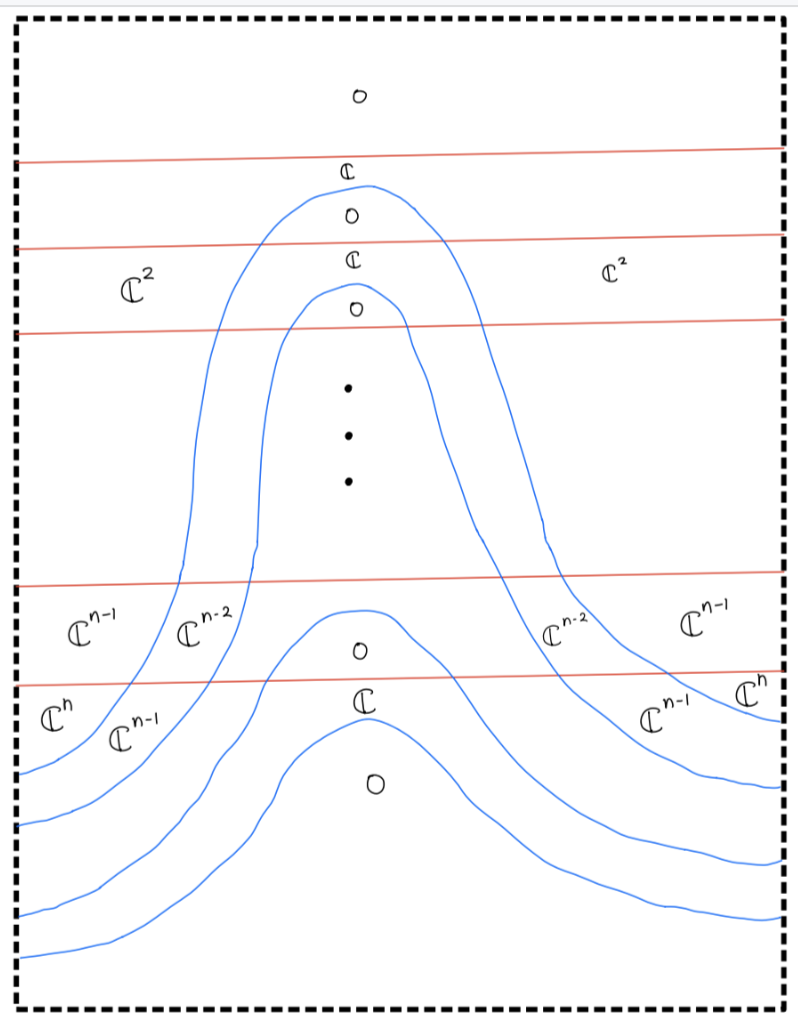
\includegraphics[scale = 0.95]{diagrams/cobord_inter/1.png}
    \caption{}
    \label{fig:your-label}
\end{figure} 

Then we define a cobordism starting from the above sheaf, say $cobord_{inter}(n)$ supported on $U$, where $n$ is the number of blue strands(equivalently red strands). At the end of the cobordism, the sheaf, under the same chart $f$, is described as the following squiggly legible diagram. 
\begin{figure}[H]
    \centering
    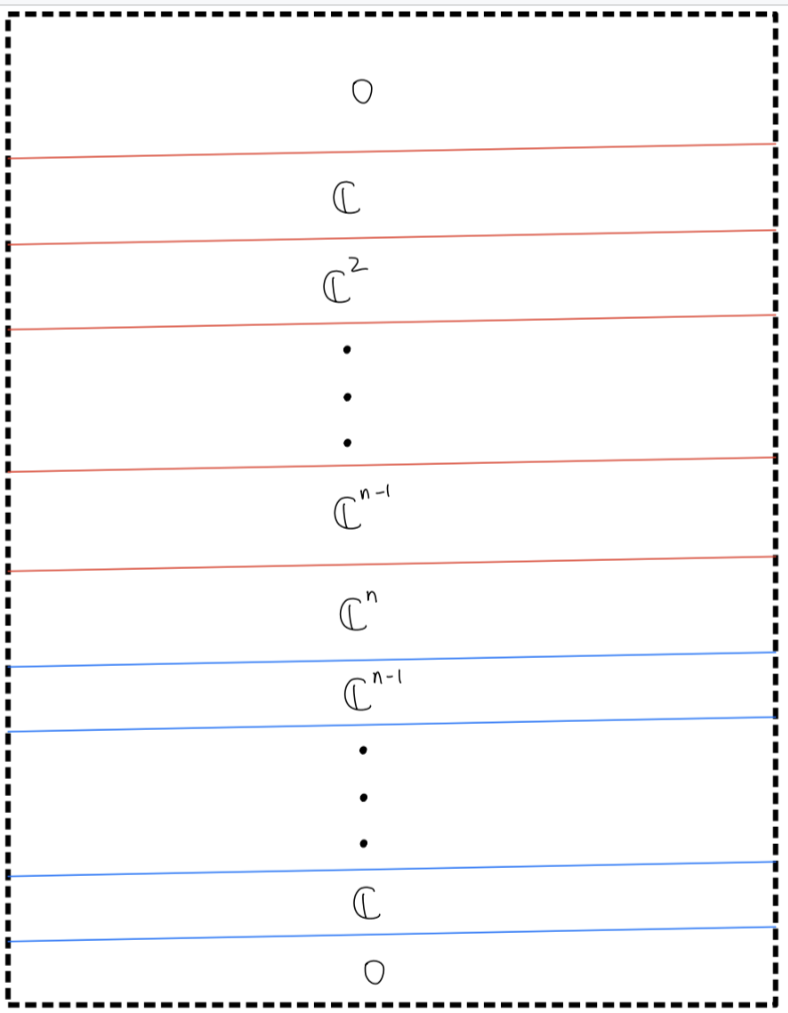
\includegraphics[scale = 0.95]{diagrams/cobord_inter/7.png}
    \caption{}
    \label{fig:your-label}
\end{figure} 
\pagebreak
We define $cobord_{inter}(n)$ inductively as follows.
\begin{enumerate}[label = (\roman*)]
\item For $n=1$, we define $cobord_{inter}(1)$ to be the null cobordism from
\begin{figure}[H]
    \centering
    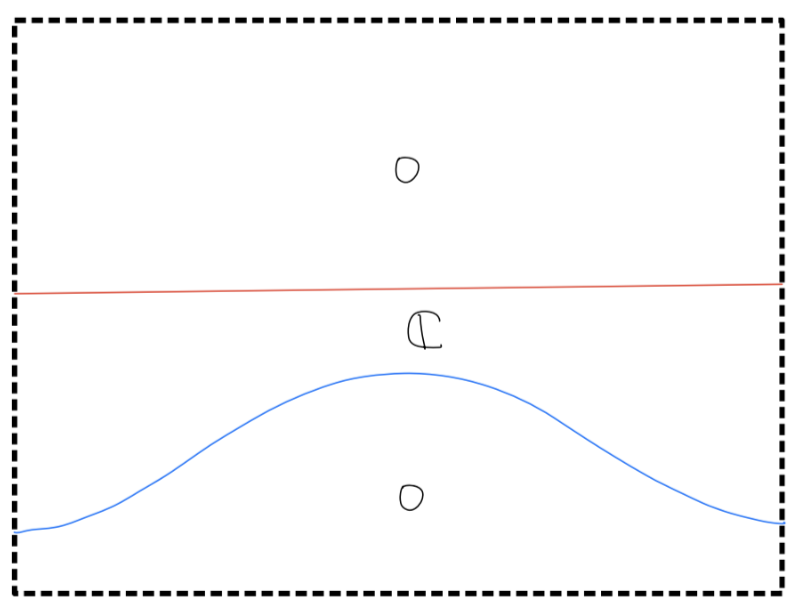
\includegraphics[scale = 0.75]{diagrams/cobord_inter/2.png}
    \caption{}
    \label{fig:your-label}
\end{figure}
to
\begin{figure}[H]
    \centering
    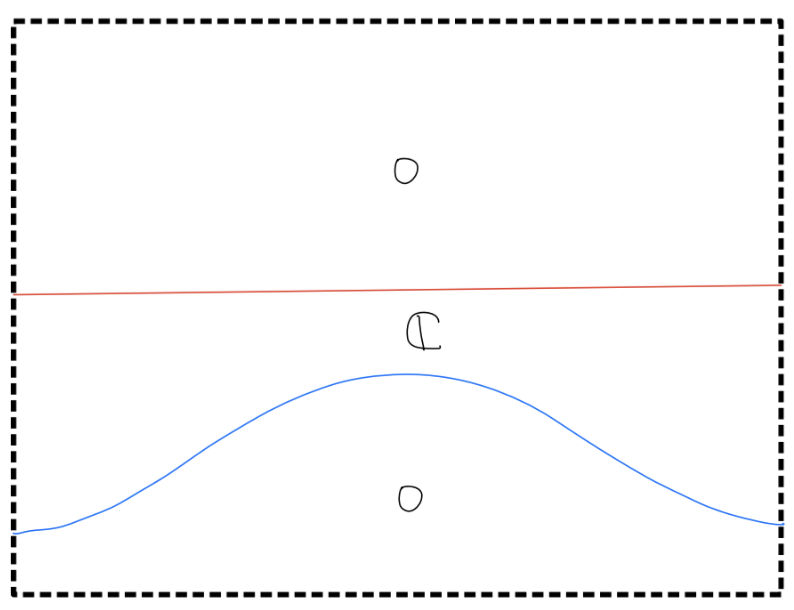
\includegraphics[scale = 0.75]{diagrams/cobord_inter/3.png}
    \caption{}
    \label{fig:your-label}
\end{figure}
\pagebreak
\item For $n>1$,
\begin{enumerate}[label = (Step \arabic*)]
\item we first apply $cobord_{inter}(n-1)$ to the square region surrounded by purple dotted lines.

\begin{figure}[H]
    \centering
    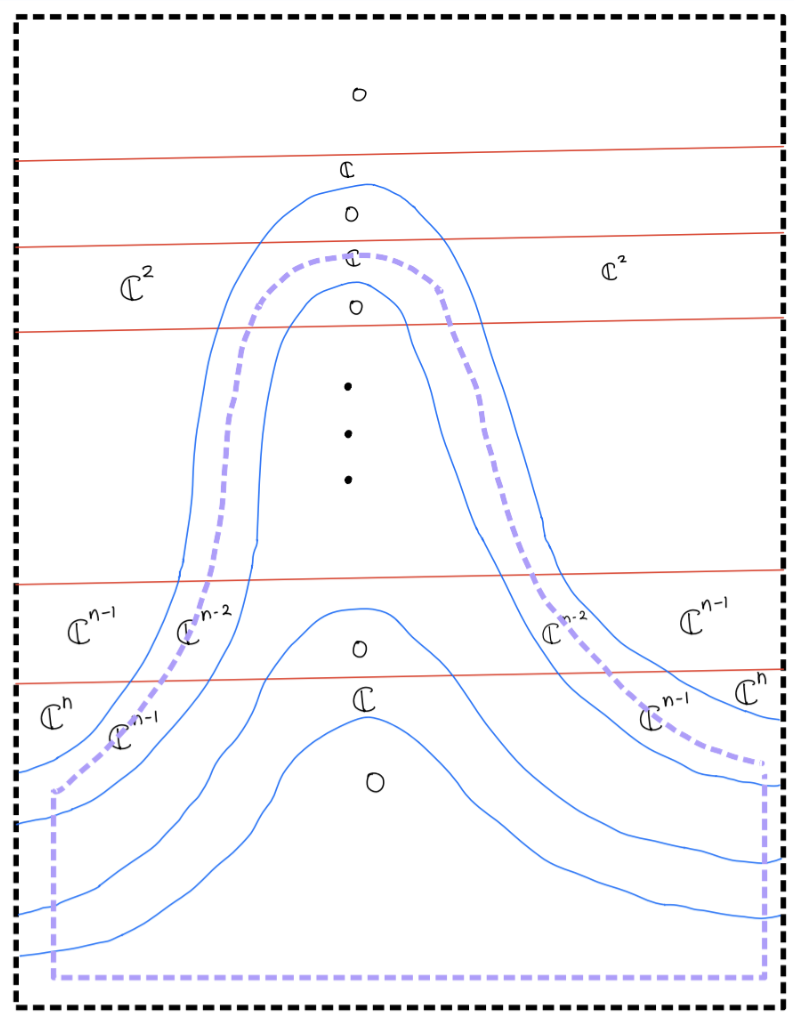
\includegraphics[scale = 0.95]{diagrams/cobord_inter/4.png}
    \caption{}
    \label{fig:your-label}
\end{figure}
\pagebreak
by induction hypothesis, we get

\begin{figure}[H]
    \centering
    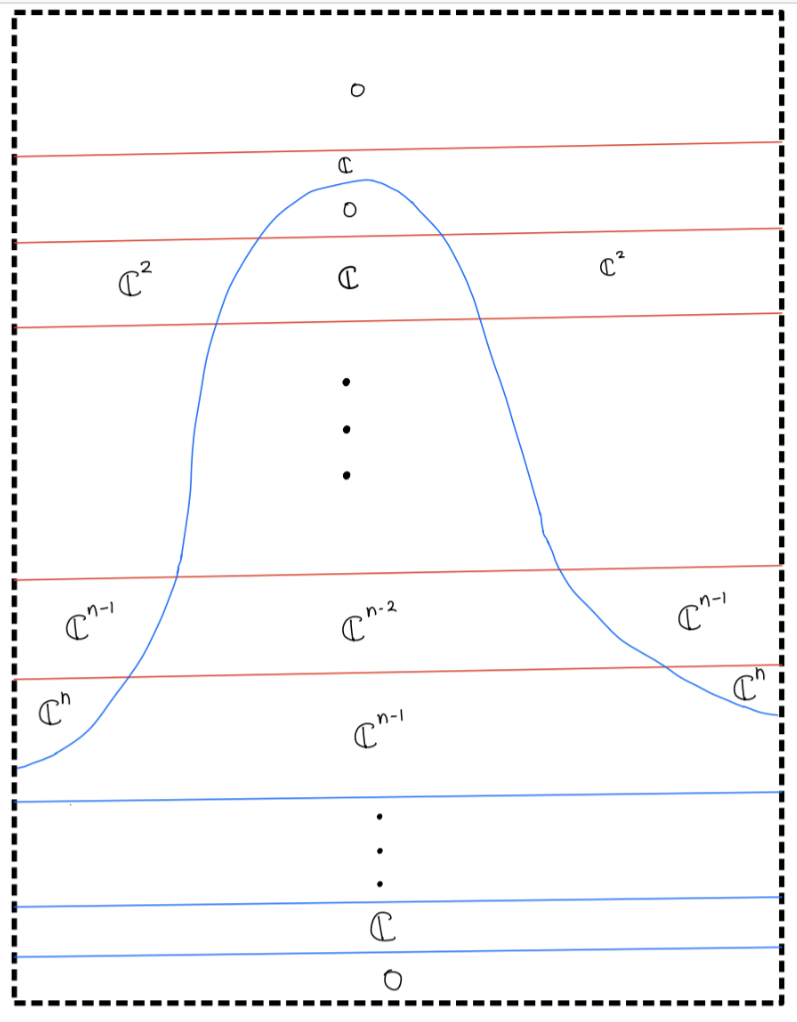
\includegraphics[scale = 0.95]{diagrams/cobord_inter/5.png}
    \caption{}
    \label{fig:your-label}
\end{figure}
\pagebreak
\item apply $cobord_7$ to the square region surrounded by purple dotted lines.

\begin{figure}[H]
    \centering
    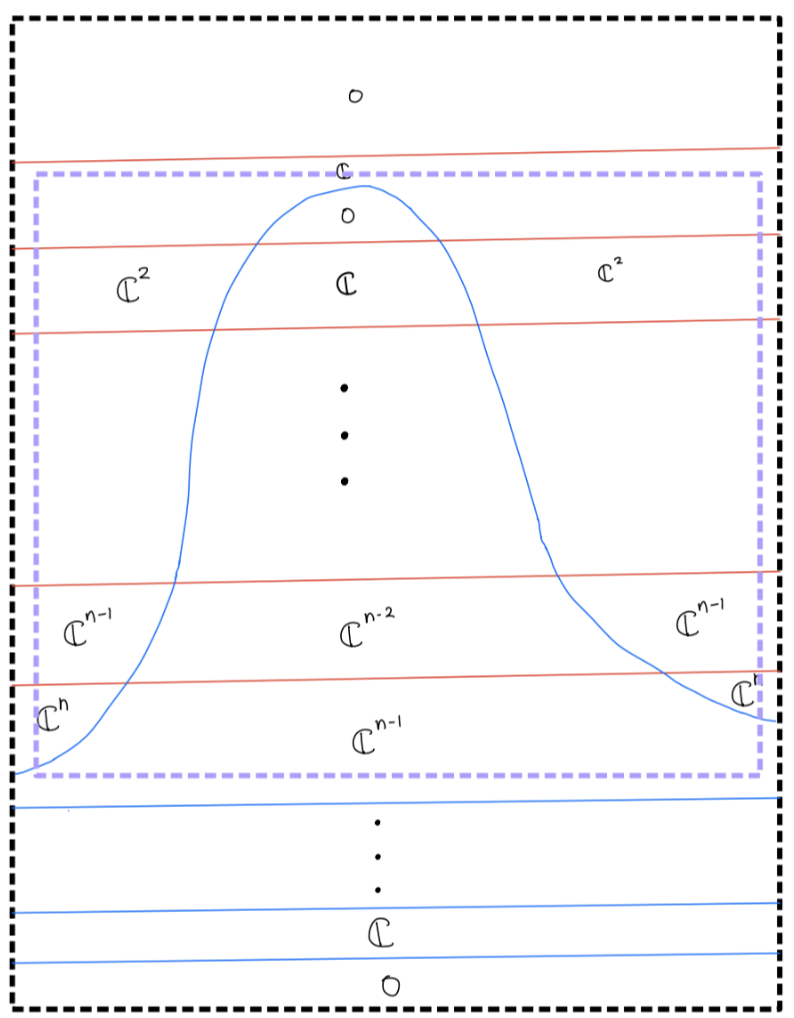
\includegraphics[scale = 0.95]{diagrams/cobord_inter/6.png}
    \caption{}
    \label{fig:your-label}
\end{figure}
\pagebreak
we get

\begin{figure}[H]
    \centering
    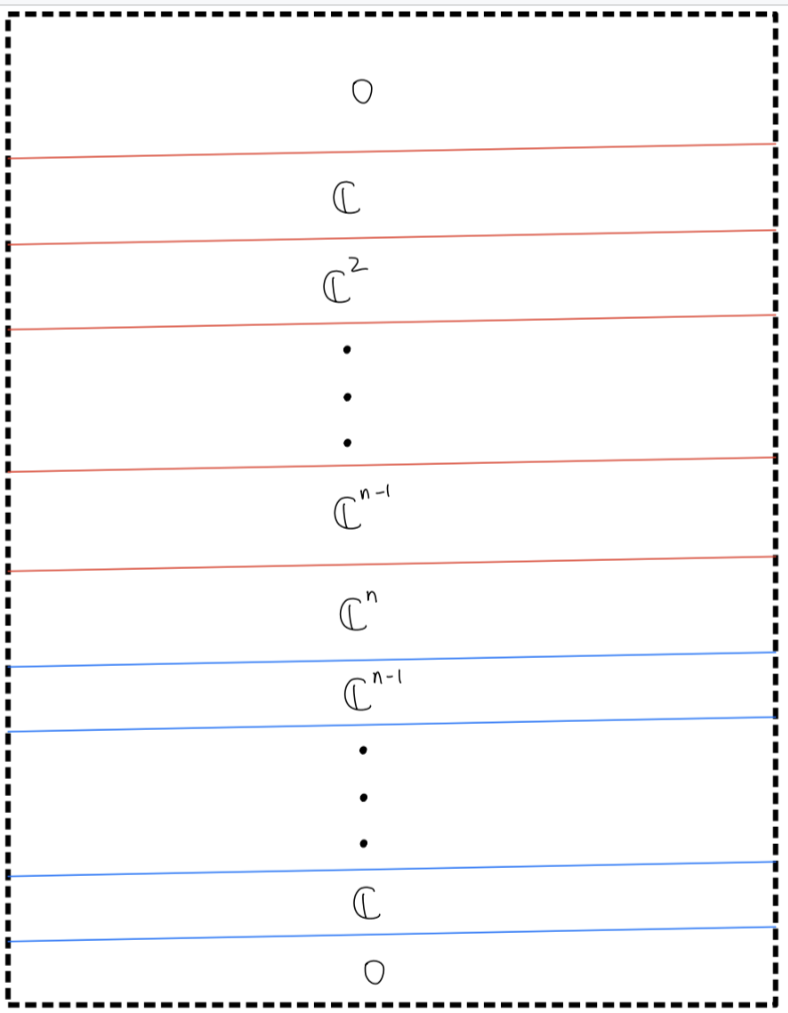
\includegraphics[scale = 0.95]{diagrams/cobord_inter/7.png}
    \caption{}
    \label{fig:your-label}
\end{figure}
\pagebreak
which is isomorphic to the final sheaf
\begin{figure}[H]
    \centering
    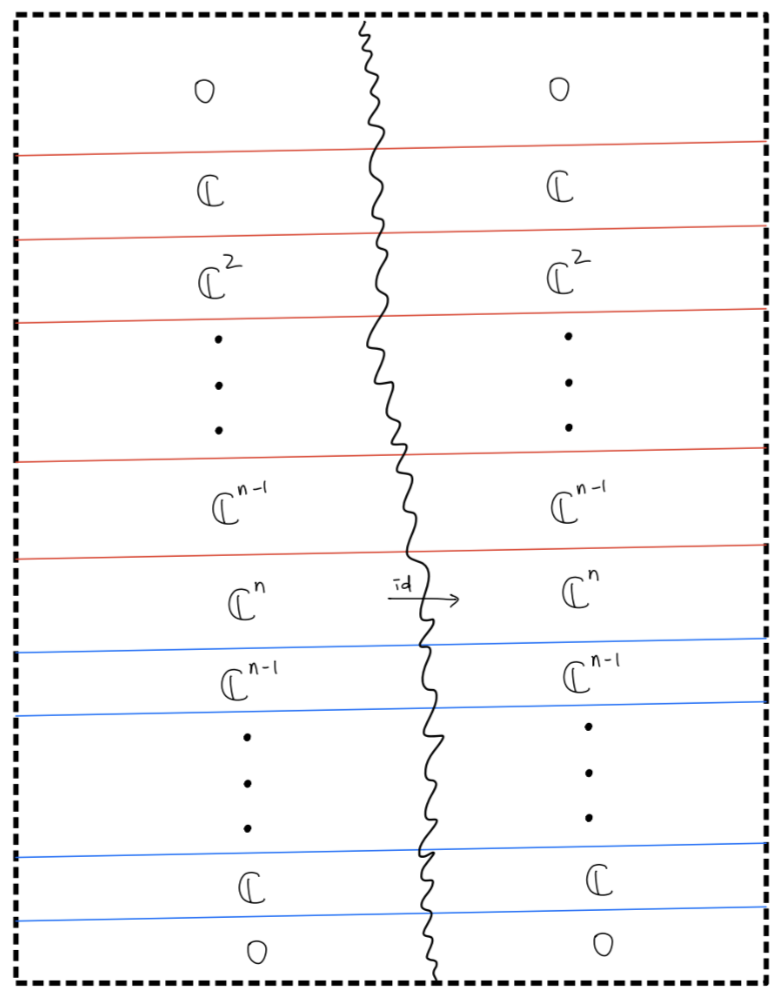
\includegraphics[scale = 0.95]{diagrams/cobord_inter/8.png}
    \caption{}
    \label{fig:your-label}
\end{figure}
\end{enumerate}
\end{enumerate}
\pagebreak